\documentclass{article}
\usepackage[T1]{fontenc}

\usepackage{graphicx}
\usepackage{listings}
\begin{document}

\title{FOSS Lab Report}
\author{Gokul K\\[2\baselineskip]
Roll Number: 21\\[2\baselineskip]}
\date{20 January 2020}

\maketitle

\setcounter{section}{1}
\section{Linux commands for operations such as redirec-
tion, pipes, filters, job control, and links.}
\subsection{Aim}
To familiarise linux commands for operations such as redirection, pipes, filters, job control, linking.
\subsection{Commands}
\subsubsection{Redirection of Standard Input/Output}
The standard input/output of a linux command can be redirected to a file. For taking input from a file the format is \begin{verbatim}
    command < file
\end{verbatim}
For printing the output of a command to an external file we use:
\begin{verbatim}
    command > file
\end{verbatim}
To take input from file1 and to print the output to file2 we can use:
\begin{verbatim}
    command < file1 > file2
\end{verbatim}
\begin{figure}[h]
    \centering
    
\includegraphics[width=.80\textwidth]{img/p2/ss1.png}
    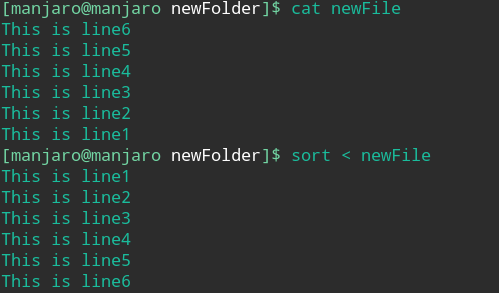
\includegraphics[width=.80\textwidth]{img/p2/ss2.png}
    \caption{Sample input/output of I/O redirection}
\end{figure}
    

\subsubsection{Pipes}
Pipes are used to feed the standard output of an command as the input of another command\newline
\hspace{\parindent} {\em usage}: \begin{verbatim} command1 | command2 \end{verbatim}
\hspace{\parindent} {\em Here the output to the command1 will be the input to command2}
\begin{figure}[h]
    \centering
    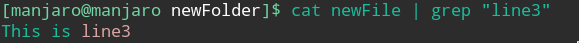
\includegraphics[width=.80\textwidth]{img/p2/ss4.png}
    \caption{Sample usage of pipes}
\end{figure}

\subsubsection{Filters}
Filters operate on the standard input and print results to the standard output. Examples of filters are
\begin{itemize}
    \item {\bf sort}: Used to sort the lines in the standard input\newline
    \item {\bf uniq}: To print unique items in a sorted input\newline
    \item {\bf grep}: Searches for a regular expression in the input\newline
    \item {\bf fmt}: Formats the standard input\newline
    \item {\bf pr}: Takes the input and provides a printer friendly output with page numbers, etc\newline
    \item {\bf head, tail}: Used to print the top and bottom portions of a file respectively\newline
    \item {\bf tr}: To transform the case of input\newline
    \begin{figure}[h!]
        \centering
        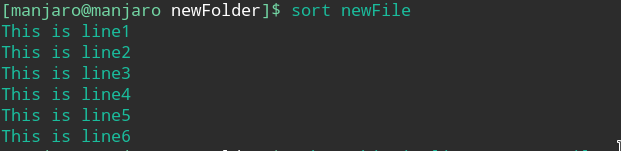
\includegraphics[width=.80\textwidth]{img/p2/ss5.png}
         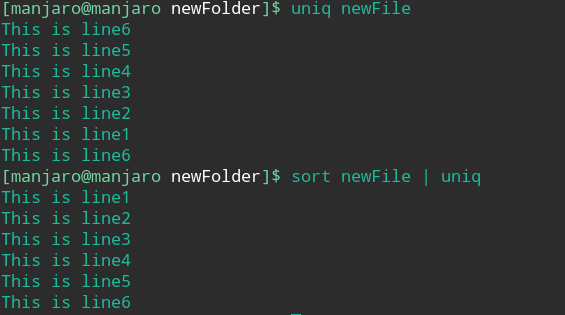
\includegraphics[width=.80\textwidth]{img/p2/ss6.png}
         
\includegraphics[width=.80\textwidth]{img/p2/ss7.png}
         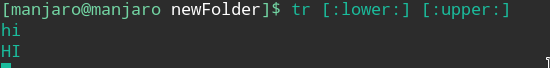
\includegraphics[width=.80\textwidth]{img/p2/ss8.png}
        \caption{Sample input/output of filter commands}
    \end{figure}
\end{itemize}

\subsubsection{Job control}
\begin{enumerate}
    \item {\bf ps}: Lists all processes running in the system\newline
    \item {\bf kill}: Used to kill a specific process in the system\newline
    \hspace{\parindent} {\em usage}: kill [options] [signal] PID\newline
    
    \item {\bf bg, fg}: Used to put a process in background/foreground respectively\newline
    \item {\bf who}: The standard Unix command who displays a list of users who are currently logged into the computer\newline
    \begin{figure}[h!]
        \centering
        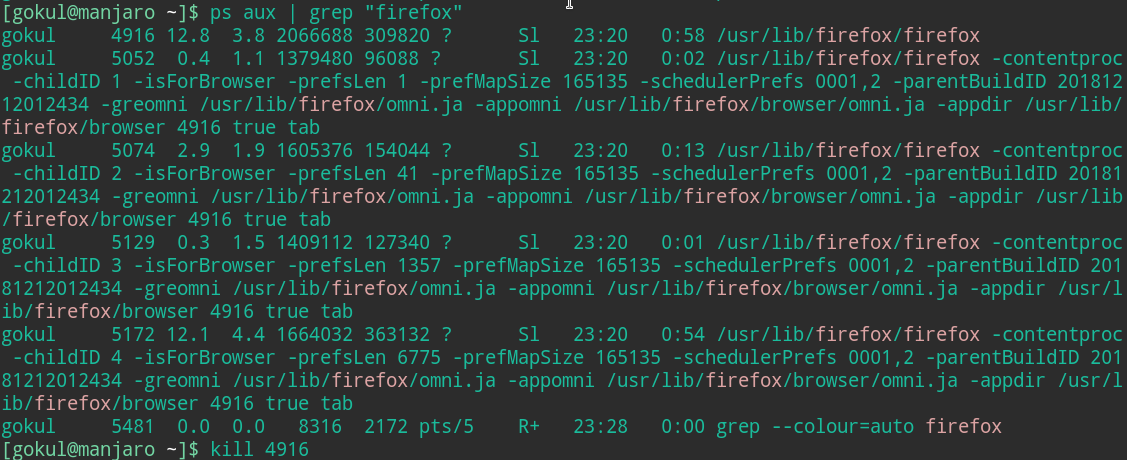
\includegraphics[width=.83\textwidth]{img/p2/ss13.png}
        \caption{Identifying the PID of firefox process and killing it}
    \end{figure}
    \begin{figure}[h!]
        \centering
        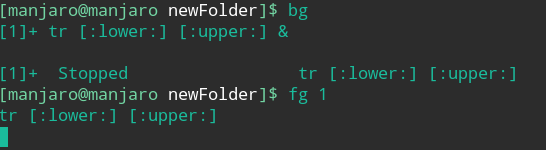
\includegraphics[width=.83\textwidth]{img/p2/ss9.png}
        \caption{fg and bg commands}
    \end{figure}
    \begin{figure}[h!]
        \centering
        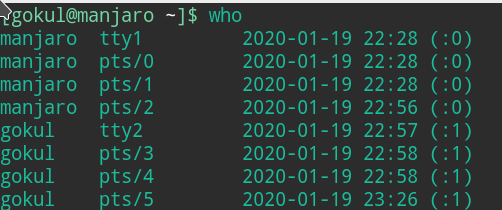
\includegraphics[width=.83\textwidth]{img/p2/ss12.png}
        \caption{who command}
    \end{figure}
\end{enumerate}

\subsubsection{Linking}
\begin{enumerate}
    \item {\bf ln}: ln command is used to link a file to another location. Two types of links are hard link and soft link. A hard linked file has existence without the source file. That is it is like two filenames pointing to the same file. A soft link works like a shortcut and when the source file is removed soft link becomes unusable s flag is used for soft linking.
    \newline
    \hspace{\parindent} {\em usage} ln [option] source destination
    
    \begin{figure}[h!]
        \centering
        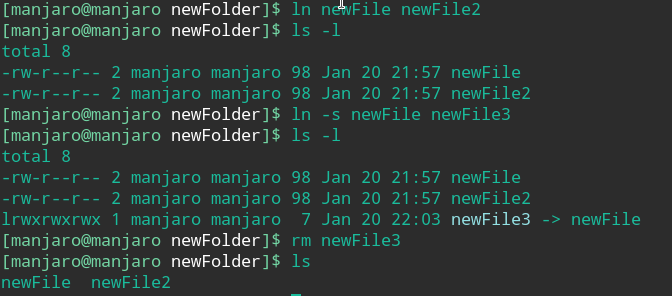
\includegraphics[width=.83\textwidth]{img/p2/ss10.png}
        \caption{Linking two files}
    \end{figure}
\end{enumerate}
\subsection{Result}
The above commands are executed and output is verified
\end{document}